\section{Virtualización de un cluster}

		\todo[inline,caption={TODO}]{Aca va la descripción de porque es importante virtualizar, para que se necesita y que es lo que se esta virtualizando.}


% http://galois.eafit.edu.co/vms/devenv/rocks-6.1/

La siguiente es la descripción de los pasos a seguir para la creación de un ambiente de pruebas paralelo virtualizado que simula el cluster de Apolo.\footnote{Estas instrucciones fueron probadas en un ambiente de Linux Fedora 18.}


\subsection{Configuración del Nodo Maestro}
\begin{enumerate}

\item Descargue e Instale VirtualBox Manager. \footnote{\url{https://www.virtualbox.org/wiki/Downloads}}

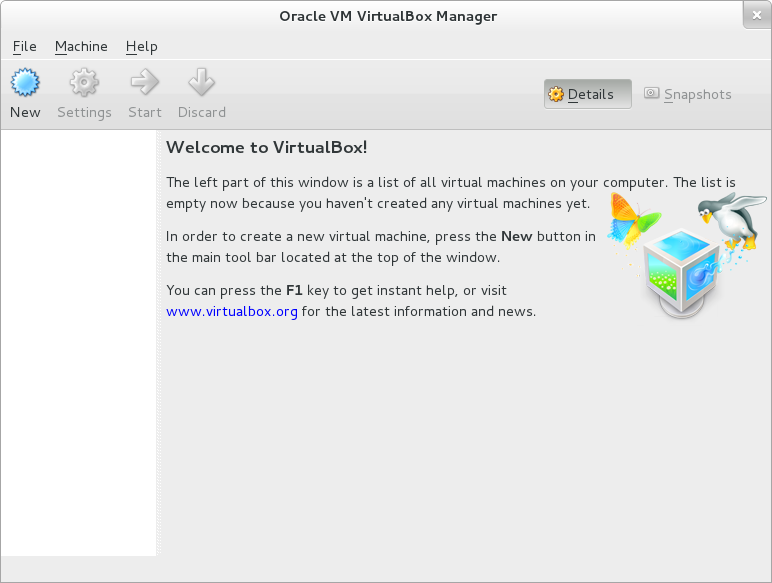
\includegraphics[width=0.5\textwidth]{aux/vb_instalado}

\item Descargar la imagen del Master.\footnote{\url{http://goo.gl/8eTJOr}}

\item Descargue el ``Extension Pack''. \footnote{\url{https://www.virtualbox.org/wiki/Downloads}}

\item Una vez instalado VirtualBox en su computador, proceda a instalar el Extensión Pack: 

	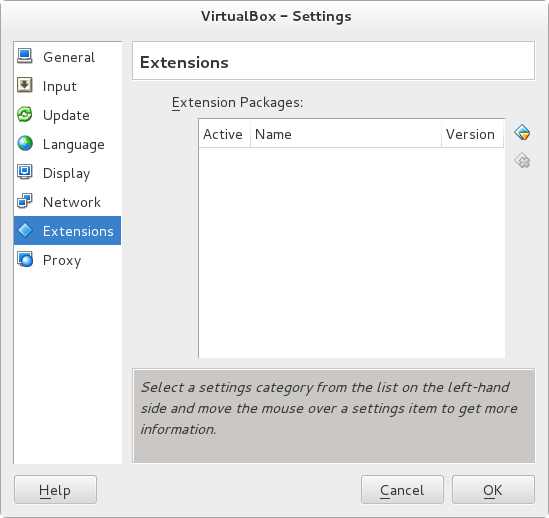
\includegraphics[width=0.5\textwidth]{aux/sinextensionpack}
	
\begin{itemize}


	\item En VirtualBox acceda al menú Archivo $\rightarrow$ Preferencias $\rightarrow$ Sección Extensiones $\rightarrow$ Proceda a instalar el ``Extension Pack''. 
	
	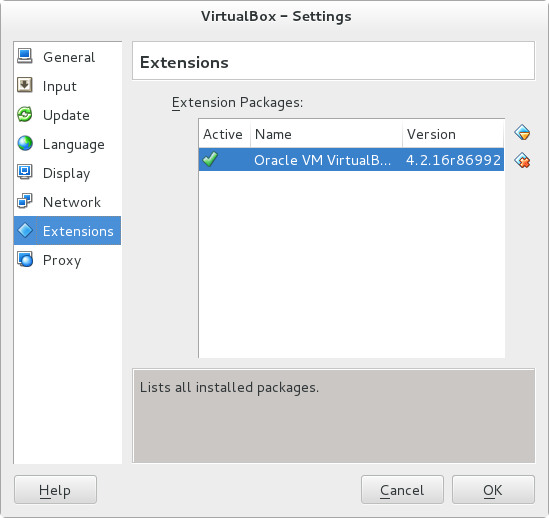
\includegraphics[width=0.5\textwidth]{aux/conextensionpack}

	\item Vaya a la sección Red $\rightarrow$ Adicione una red Sólo Anfitrión. Esta debe ser la primera interfaz de red de Sólo Anfitrión que se crea, si ya está creada por favor no cree otra adicional.


	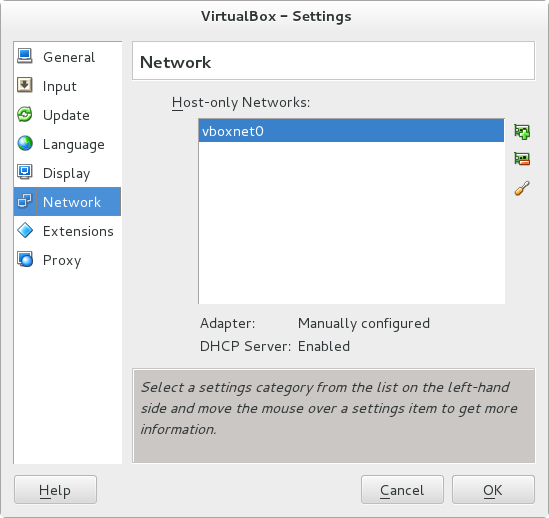
\includegraphics[width=0.5\textwidth]{aux/hostonly}
	

	\item Haga click en aceptar para finalizar la operación.

\end{itemize}

\item En VirtualBox, importe desde el Menú $\rightarrow$ Importar Appliance. Deje la configuración por defecto y \textbf{no} reinicialice la dirección MAC.


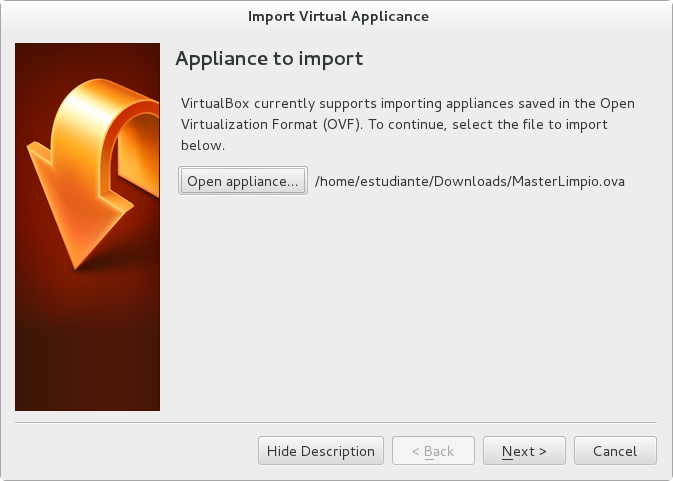
\includegraphics[width=0.5\textwidth]{aux/importappliance}


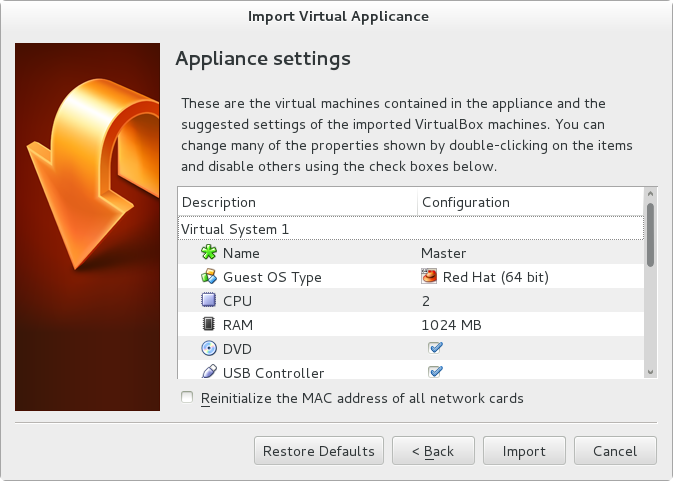
\includegraphics[width=0.5\textwidth]{aux/applianceops1}

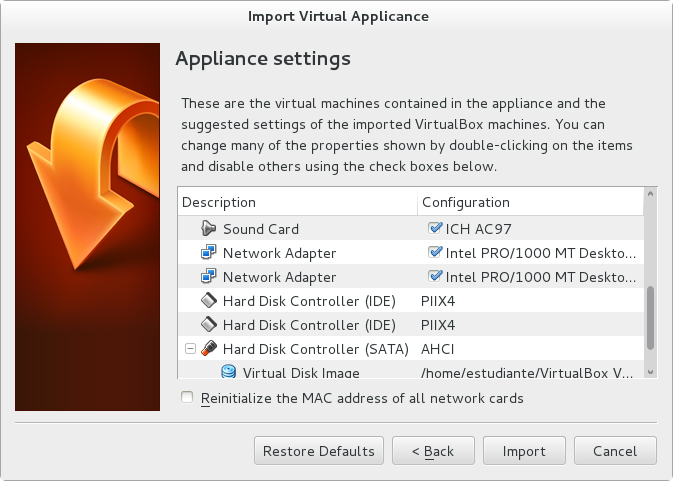
\includegraphics[width=0.5\textwidth]{aux/applianceops2}


\item Señale la máquina virtual llamada ``Master'' y vaya a la configuración y revise la siguiente configuración en esta:

\begin{itemize}

	\item En la sección Sistema, pestaña Procesador, debe tener dos procesadores y habilitado PAE/NX.

	
	
	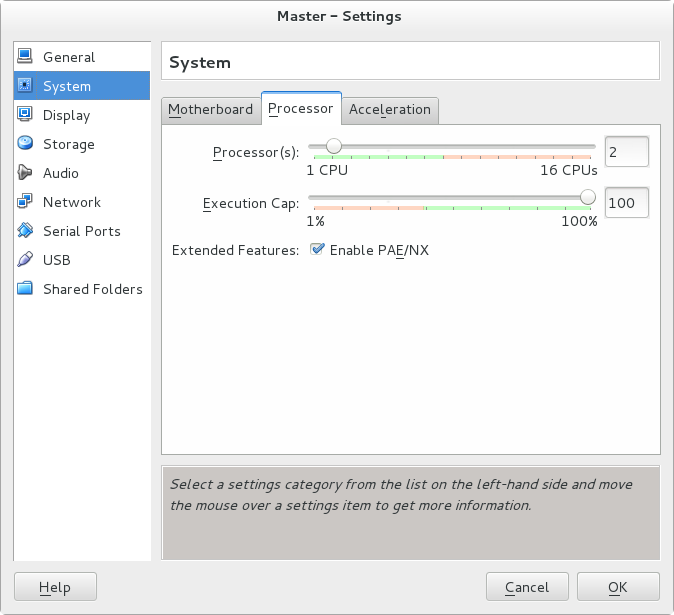
\includegraphics[width=0.5\textwidth]{aux/procesadores}
	

	\item En la sección Red, pestaña Adaptador 1, deberá estar configurado como NAT. 


	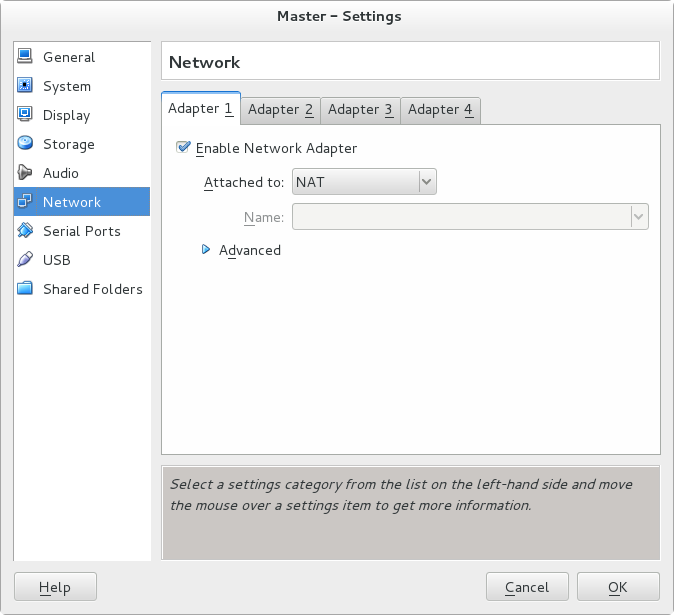
\includegraphics[width=0.5\textwidth]{aux/rednat}
	

	\item En la pestaña Adaptador 2 deberá estar en Adaptador Sólo--Anfitrión y el nombre deberá ser \texttt{vboxnet0}\footnote{Tenga en cuenta que este adaptador se llama \texttt{vboxnet0} en Linux, en Windows tendrá otro nombre, lo más importante es que sea la primera interfaz de red de Sólo Anfitrión, ya que sino dará lugar al problema de reasignación de interfaces de red dentro del nodo Master, en otras palabras, asignará las interfaces eth2 y eth3 en vez de asignar eth0 y eth1 a la NAT y a la Sólo Anfitrión respectivamente.}.


	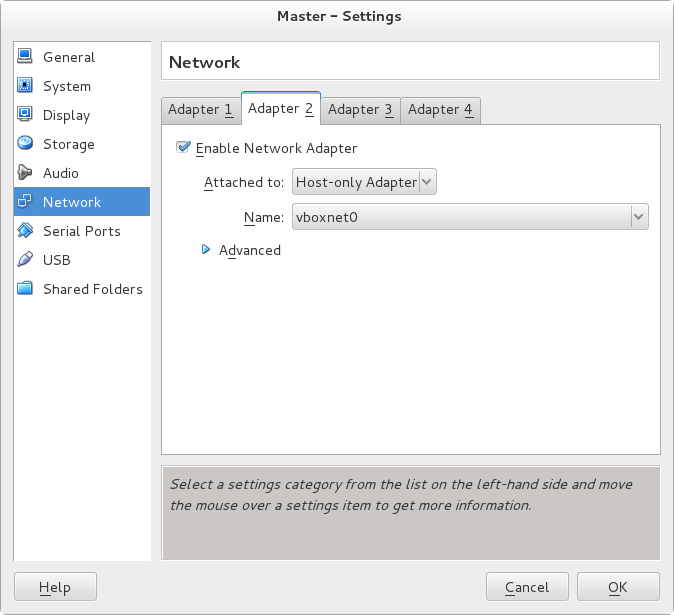
\includegraphics[width=0.5\textwidth]{aux/redhost}
	

	\item Acepte todos los cambios.

\end{itemize}

\item Señale la máquina Master e iníciela.

\item Una vez iniciada la máquina virtual del Master proceda a crear una nueva máquina virtual como Nodo Trabajador a partir de los siguientes pasos:

\begin{itemize}
	\item Haga click en Crear Nueva Máquina.

	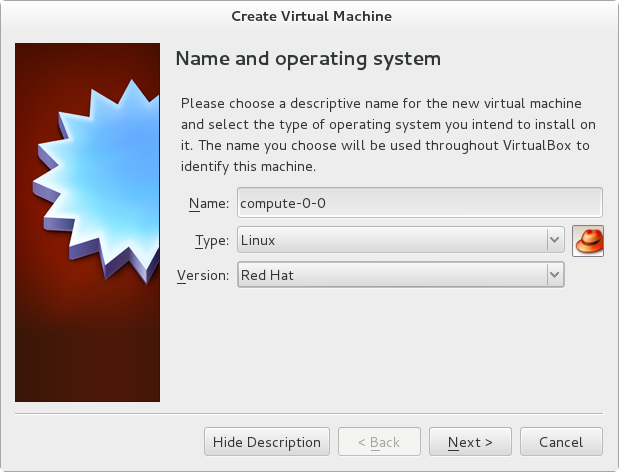
\includegraphics[width=0.5\textwidth]{aux/opcnodo1}

	\item El nombre será \textit{compute-0-0}.

	\item El tipo será Linux.

	\item La versión será Red Hat de 64 bits.

	

	\item Click en siguiente.

	\item Asigne 1024 Megabytes de Memoria RAM\footnote{La cantidad de memoria RAM asignada será proporcional a la que tenga el sistema en el cual están las máquinas virtuales. Igual con el disco duro y los procesadores, sin embargo, para efectos de ver la paralelización en memoria compartida se recomienda tener 2 procesadores por máquina}.

	\item Cree el disco duro con 30 gigas de espacio, recuerde que esto se asignará dinámicamente. El tipo de disco duró será VDI y dinámicamente asignado.



	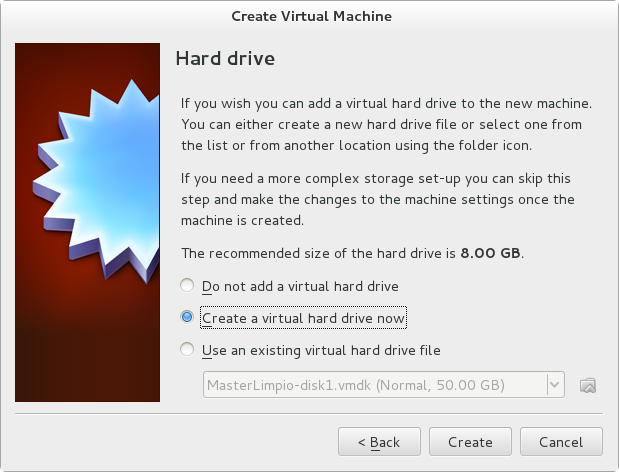
\includegraphics[width=0.5\textwidth]{aux/nodohd}

	
	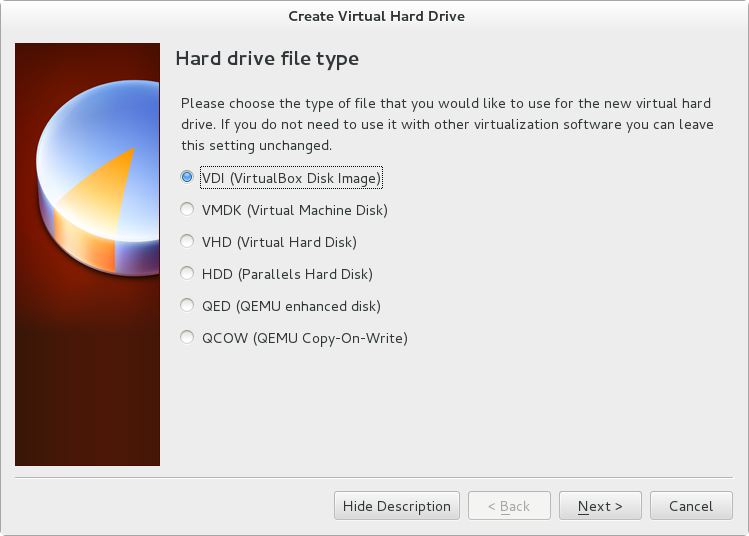
\includegraphics[width=0.5\textwidth]{aux/nododvi}


	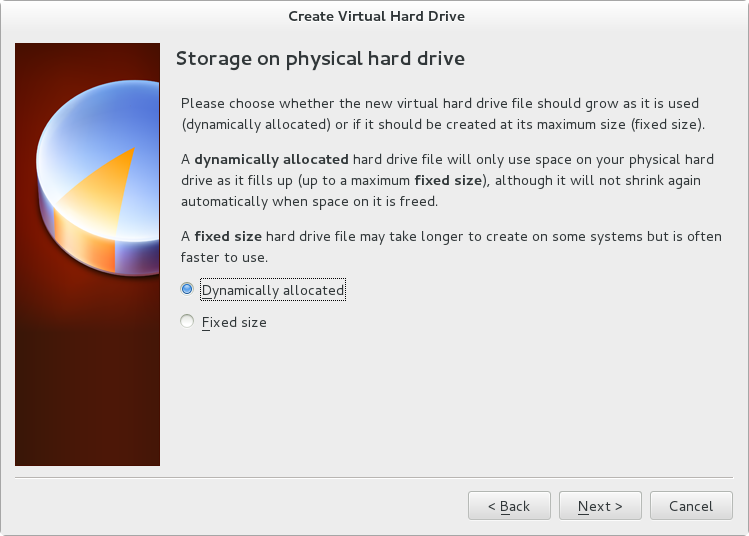
\includegraphics[width=0.5\textwidth]{aux/hddinamico}


	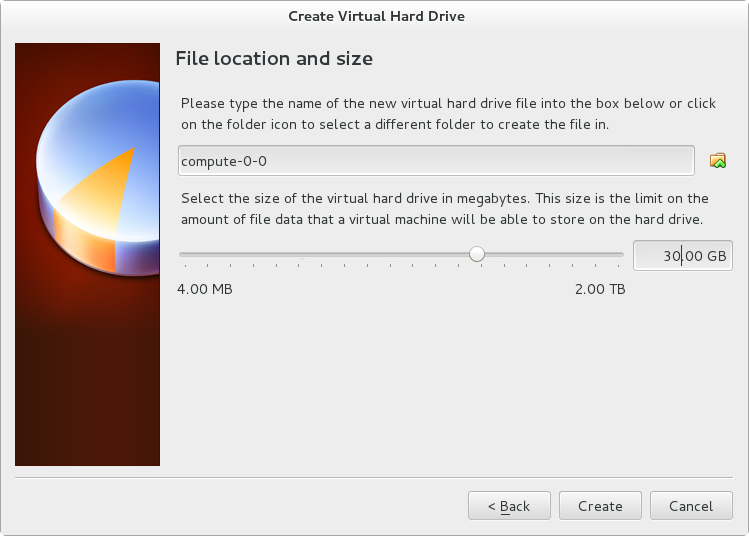
\includegraphics[width=0.5\textwidth]{aux/nodohdsize}
	

\end{itemize}

\item Una vez creado el nodo trabajador se procede a configurarlo a partir de los siguientes pasos:

\begin{itemize}
	\item Señalar la máquina \textit{compute-0-0} y dar click en Configurar.

	\item En la pestaña Sistema, asegúrese de que tenga la cantidad de memoria RAM correcta

	\item Deshabilite el \textit{floppy disk}

	\item habilite la red como dipositivo de \textit{booteo} y además súbalo como primer dispositivo, sólo deberá quedar la tarjeta de red como primera opción y como segunda el disco duro de la máquina virtual, de esta manera nos aseguramos que esta máquina virtual pueda instalarse automáticamente de manera desatendida, por esta razón el clúster es escalable. 

	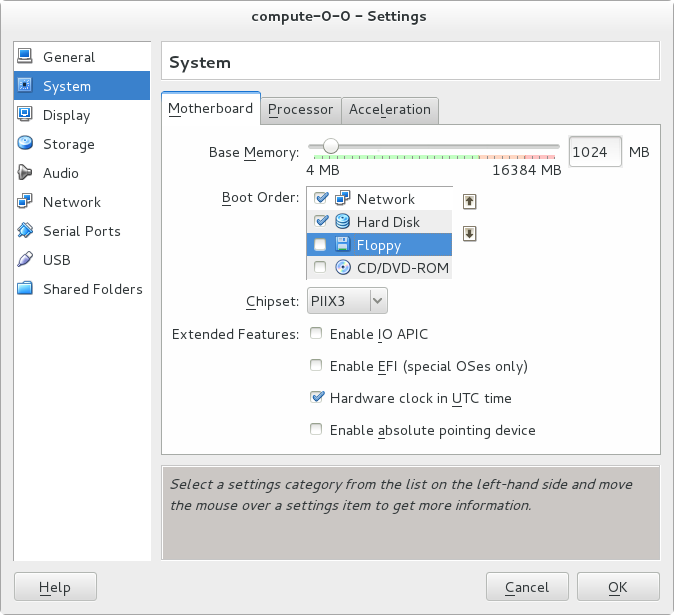
\includegraphics[width=0.5\textwidth]{aux/nodoopsboot}


	\item En la pestaña Procesador asegúrese de que hay dos procesadores y está habilitado PAE/NX.


	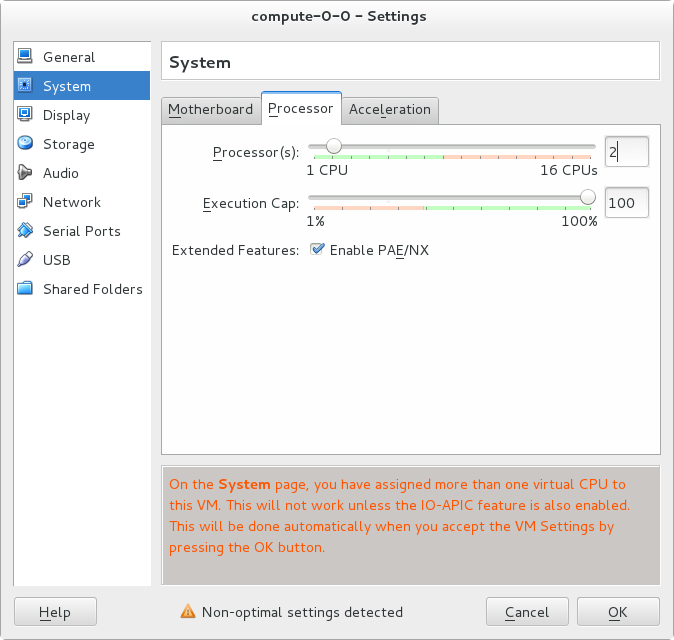
\includegraphics[width=0.5\textwidth]{aux/nodoprocesadores}
	

	\item En la sección Red deberá configurar sólo la primera interfaz de red y deberá estar configurada como Sólo--Anfitrión y deberá tener \texttt{vboxnet0}.


	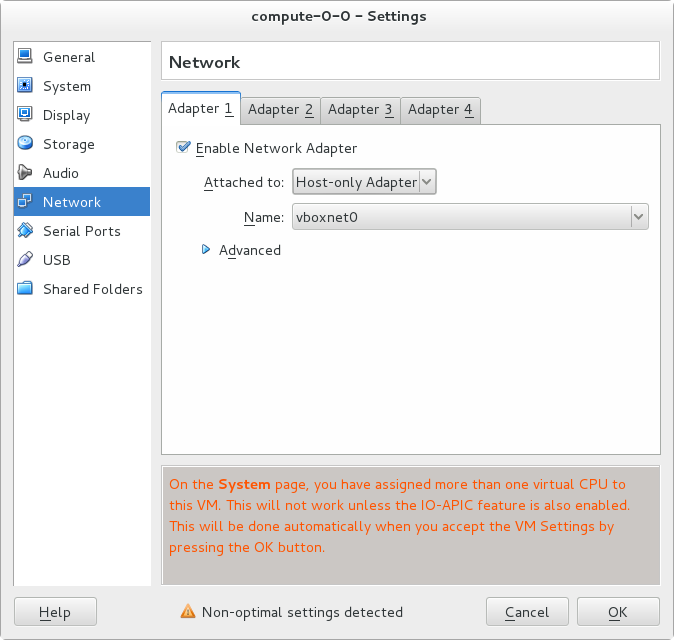
\includegraphics[width=0.5\textwidth]{aux/nodored}
	

	\item Acepte los cambios.
\end{itemize}


\item Repita los pasos para crear otro nodo si lo considera necesario para crear el \textit{compute-0-1}, siempre y cuando la computadora que usted tiene soporte una tercera máquina virtual ejecutandose al tiempo que el Nodo Master y el \textit{compute-0-0}

\item Ingrese en el Nodo Master como usuario \texttt{root} y la contraseña es \texttt{apolito123!}

\item Abra una consola

\item Ingrese el comando \texttt{insert-ethers}

\item Escoja \texttt{Compute}. Aparecerá una interfaz de consola mostrándole los nodos agregados en la medida que se les vaya asignando IP por medio de DHCP y una imagen de Linux para instalar con PXE.

\item Encienda de uno en uno los Nodos trabajadores que haya creado, empezando por el \textit{compute-0-0} y así sucesivamente. Observará que aparece en la interfaz \texttt{insert-ethers} la dirección MAC del Nodo Trabajador, se le asignará el nombre compute-0-0 y si aparece un símbolo de asterísco es porque recibió exitosamente la imagen para la instalación de Linux.

\item Una vez de que los nodos se termine de instalar automáticamente salga de la interfaz de \texttt{insert-ethers} en el Master con la tecla F8.

\item Ingrese al directorio especificado con el siguiente comando: \texttt{cd /export/apps/installers}

\item Descargue el instalador del comando \texttt{htop} con la siguiente instrucción: \texttt{wget http://goo.gl/TDWExw}

\item Instale \texttt{htop} en el nodo Master con la siguiente instrucción: \texttt{rpm -ivh htop*.rpm}

\item Ahora instale masivamente \texttt{htop} en el resto del clúster con el siguiente comando: \texttt{rocks run host ``rpm -ivh /share/apps/installers/htop*.rpm''}

\item El cluster está completo.

\end{enumerate}

\subsection{Configuración de los Nodos Esclavos}

\begin{enumerate}
	\item Una vez que se tiene el nodo Master funcionando y por lo menos un nodo trabajador como el \textit{compute-0-0} se procede a realizar los siguientes pasos de configuración:

	\begin{itemize}
	\item Adicione un usuario sin privilegios con los siguientes comandos\footnote{En adelante el usuario de ejemplo será jdpinedac, pero usted podrá asignar el nombre de usuario que desee}:

	\begin{itemize}
		\item \textbf{\texttt{adduser jdpinedac}} Para crear un usuario sin privilegios.

		\item \textbf{\texttt{passwd jdpinedac}} Para cambiar la contraseña del usuario.

		\item \textbf{\texttt{rocks sync users}} Para sincronizar el usuario creado en todo el cluster, este usuarió estará creado tanto en el nodo master como en los nodos trabajadores.
	\end{itemize}

	\item \textit{su - jdpinedac} Para que el usuario \texttt{root} se convierta en el usuario sin privilegios. Se le harán algunas preguntas de contraseñas, déjelas vacías presionando la tecla \textit{enter} varias veces.
	\end{itemize}
	
\end{enumerate}


\section{Preguntas Frecuentas:}[Posibles Problemas]

\begin{itemize}
	\item Los nodos de trabajo no inician Correctamente: Es posible que estos hayan sido apagados de manera incorrecta. 
	siga el procedimiento desde el numeral X hasta el Y de ``ASDF''

	\item Verifique que su computador puede virtualizar: Ingrese a la BIOS y verifique que esta activida la opcion de Virtualización de Hardware. 

	\item Si su caso no se encuentra aqui listado contacte al autor
\end{itemize}